\documentclass[11pt]{article}
\usepackage{a4wide}
\usepackage{longtable}
\usepackage{amssymb,url}
\usepackage{graphicx}
\usepackage{latexsym}
\usepackage{tikz}
\usepackage{tikz,tkz-tab,amsmath}
\usepackage{tikzrput}
\usepackage{fancyvrb}
\usepackage{booktabs}
\usepackage{multirow} 
\usepackage{textcomp}
\usepackage{siunitx}
\usepackage[colorlinks=true,citecolor=blue]{hyperref}
\usepackage[tableposition=below]{caption}
\captionsetup[longtable]{skip=1em}


\title{Complementary Experiments of the Thick Line Segment Detection Algorithm: Evaluation of ADS and ATC Concepts}
\date{
  $^1$ Universit\'e de Lorraine, LORIA (UMR 7503), Nancy, France \\
  \texttt{philippe.even@loria.fr},
  \texttt{hoai-diem-phuc.ngo@loria.fr}\\
  $^2$  Universit\'e Lyon 2, LIRIS (UMR 5205), Lyon, France\\
  \texttt{bertrand.kerautret@univ-lyon2.fr}}
\author{Philippe Even $^1$ \and Phuc Ngo $^1$ \and Bertrand Kerautret $^2$}

\begin{document}

\maketitle



\abstract{This document presents complementary experiments on the
  published algorithm of Thick Line Segment Detection with Fast
  Directional Tracking. The main paper is actually published at ICIAP
  2019 \cite{Even19}.
%
First tests compare the performance of the detector with and without
adaptive directional scans (ADS) and assigned thickness control (ATC).
On the detector without ADS, the fine tracking step must be performed
twice to get less risk of growing blurred segment escape from the scan
strip.}




\section{Experimentations on synthesized images}
These tests compare both versions on a set of 1000 synthesized images containing
10 randomly placed input segments with random width between 2 and 5 pixels.
The absolute value of the difference of each found segment to its matched input segment is measured.
On these groundtruth image, the numerical error on the gradient extraction biases the line width measures.
This bias was first estimated using 1000 images containing only one input segment (no possible interaction) and the found value (1.4 pixel) was taken into account in the test.
Results are given in the following table. \\

If we call $S$ the count of pixels of all input segments in an image,
$D$ the count of pixels of all output blurred segments,
and $I$ the count of successfully detected pixels ($D \cap S$),
the given measures are:
\begin{enumerate}
\item the count of output blurred segments,
\item the count of output long ($>$ 40 pixels) blurred segments,
\item the count of undetected input segments,
\item the precision $P = I/D$,
\item the recall $R = I/S$,
\item the F-measure $F = 2.P.R / (P+R)$,
\item the absolute value of the width difference between matched output segments with input segments,
\item the absolute value of the angle difference between matched output segments with input segments.
\end{enumerate}

\pagebreak

\begin{figure}
  \begin{tabular}{ccc}
    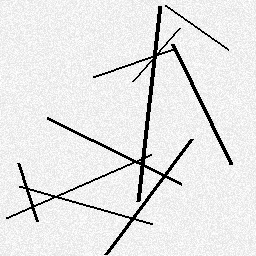
\includegraphics[width=0.3\textwidth]{Images/randimage1.png}&
    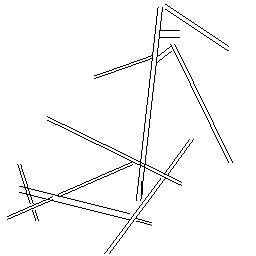
\includegraphics[width=0.3\textwidth]{Images/randold1.png}&
    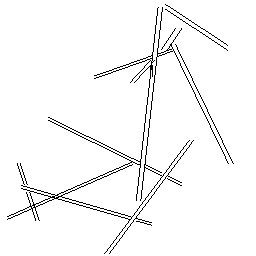
\includegraphics[width=0.3\textwidth]{Images/randnew1.png} \\
    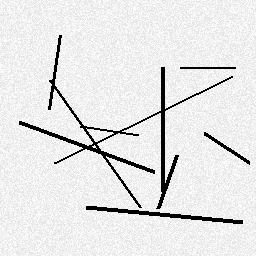
\includegraphics[width=0.3\textwidth]{Images/randimage2.png}&
    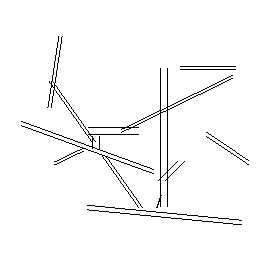
\includegraphics[width=0.3\textwidth]{Images/randold2.png}&
    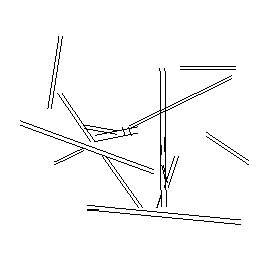
\includegraphics[width=0.3\textwidth]{Images/randnew2.png}
    \begin{picture}(1,1)(0,0)
      \put(-320,141.5){\circle{10}}
      \put(-322.5,139){a}
      \put(-175,141.5){\circle{10}}
      \put(-177.5,139){b}
      \put(-30,141.5){\circle{10}}
      \put(-32.5,139){c}
      \put(-320,5.5){\circle{10}}
      \put(-322.5,3){d}
      \put(-175,5.5){\circle{10}}
      \put(-177.5,3){e}
      \put(-30,5.5){\circle{10}}
      \put(-32.5,3){f}
    \end{picture} \\
  \end{tabular}
  \caption{Evaluation on synthesized images: two of the
  randomly generated images (a,d), bounding lines of output blurred
  segments without (b,e) and with (c,f) ADS and ATC concepts.}
  \label{fig:synth}
\end{figure}

\begin{longtable}[]{@{}l||rr|rr|rr@{}}
\toprule
& \multicolumn{2}{c|}{On Fig.~1a} & \multicolumn{2}{c|}{On Fig.~1d}
& \multicolumn{2}{c}{On whole set} \tabularnewline
ADS \& ATC Concepts & \multicolumn{1}{c}{without} & \multicolumn{1}{c|}{with}
& \multicolumn{1}{c}{without} & \multicolumn{1}{c|}{with}
& \multicolumn{1}{c}{without} & \multicolumn{1}{c}{with} \tabularnewline
\midrule
Detected blurred segments & 16 & 17 & 14 & 18 & 17.06
\textpm 3.22 &
16.83 \textpm
3.11\tabularnewline
Detected long segments & 11 & 8 & 10 & 10 & 11.24
\textpm 1.94 &
11.36 \textpm
1.97\tabularnewline
Undetected input segments & 0 & 0 & 1 & 0 & 0.152
\textpm 0.43 &
0.003 \textpm
0.05\tabularnewline
Precision (\%) & 76.30 & 85.47 & 75.38 & 83.41 & 80.46
\textpm 7.22 &
83.87 \textpm
6.04\tabularnewline
Recall (\%) & 89.81 & 93.51 & 90.88 & 91.47 & 90.23
\textpm 3.30 &
91.15 \textpm
2.52\tabularnewline
F-measure (\%) & 82.51 & 89.31 & 82.40 & 87.26 & 84.87
\textpm 4.42 &
87.23 \textpm
3.59\tabularnewline
Thickness difference (pixels) & 0.95 & 0.68 & 1.15 & 0.65 & 0.70
\textpm 0.24 &
0.59 \textpm
0.19\tabularnewline
Angle difference (degrees) & 1.11 & 0.71 & 1.99 & 1.03 & 0.61
\textpm 0.66 &
0.57 \textpm
0.62\tabularnewline
\bottomrule
\caption{Measured performance on both Figure 1 image examples and on
a whole 1000 synthesized images set, without and with adaptive directional
scans and assigned width control.}
\label{tab:synth}
\end{longtable}

\pagebreak

\section{Experimentations on real images}

Next tests compare both versions on real images:
\begin{itemize}
\item first the set of 102 images of York Urban data base \cite{Denis08}
augmented with manually extracted groundtruth lines (an example in
Fig.~\ref{fig:york}),
\item then selected images for more detailed visual analysis
(Fig.~\ref{fig:office} and Fig.~\ref{fig:castle}).
\end{itemize}
Reported measures in Tab.~\ref{tab:york}, Tab.~\ref{tab:office} and
Tab.~\ref{tab:castle}
are execution time $T$, groundtruth covering
ratio $C$ (only for the York Urban data base), number of output line
segments $N$, mean length of output line segments $L/N$, and mean
thickness of output line segments $W$. \\

Shorter execution time is achieved with the new concepts.
Detected blurred segments are shorter but thinner.
Obviously the constant assigned thickness augments the probability to extend
the segments with outlier edge points as can be noticed in the detail of
office (Fig.~\ref{fig:office}) and castle images (Fig.~\ref{fig:castle}).
Moreover, brick joints are better detected in castle image.

\begin{figure}[h]
  \begin{center}
  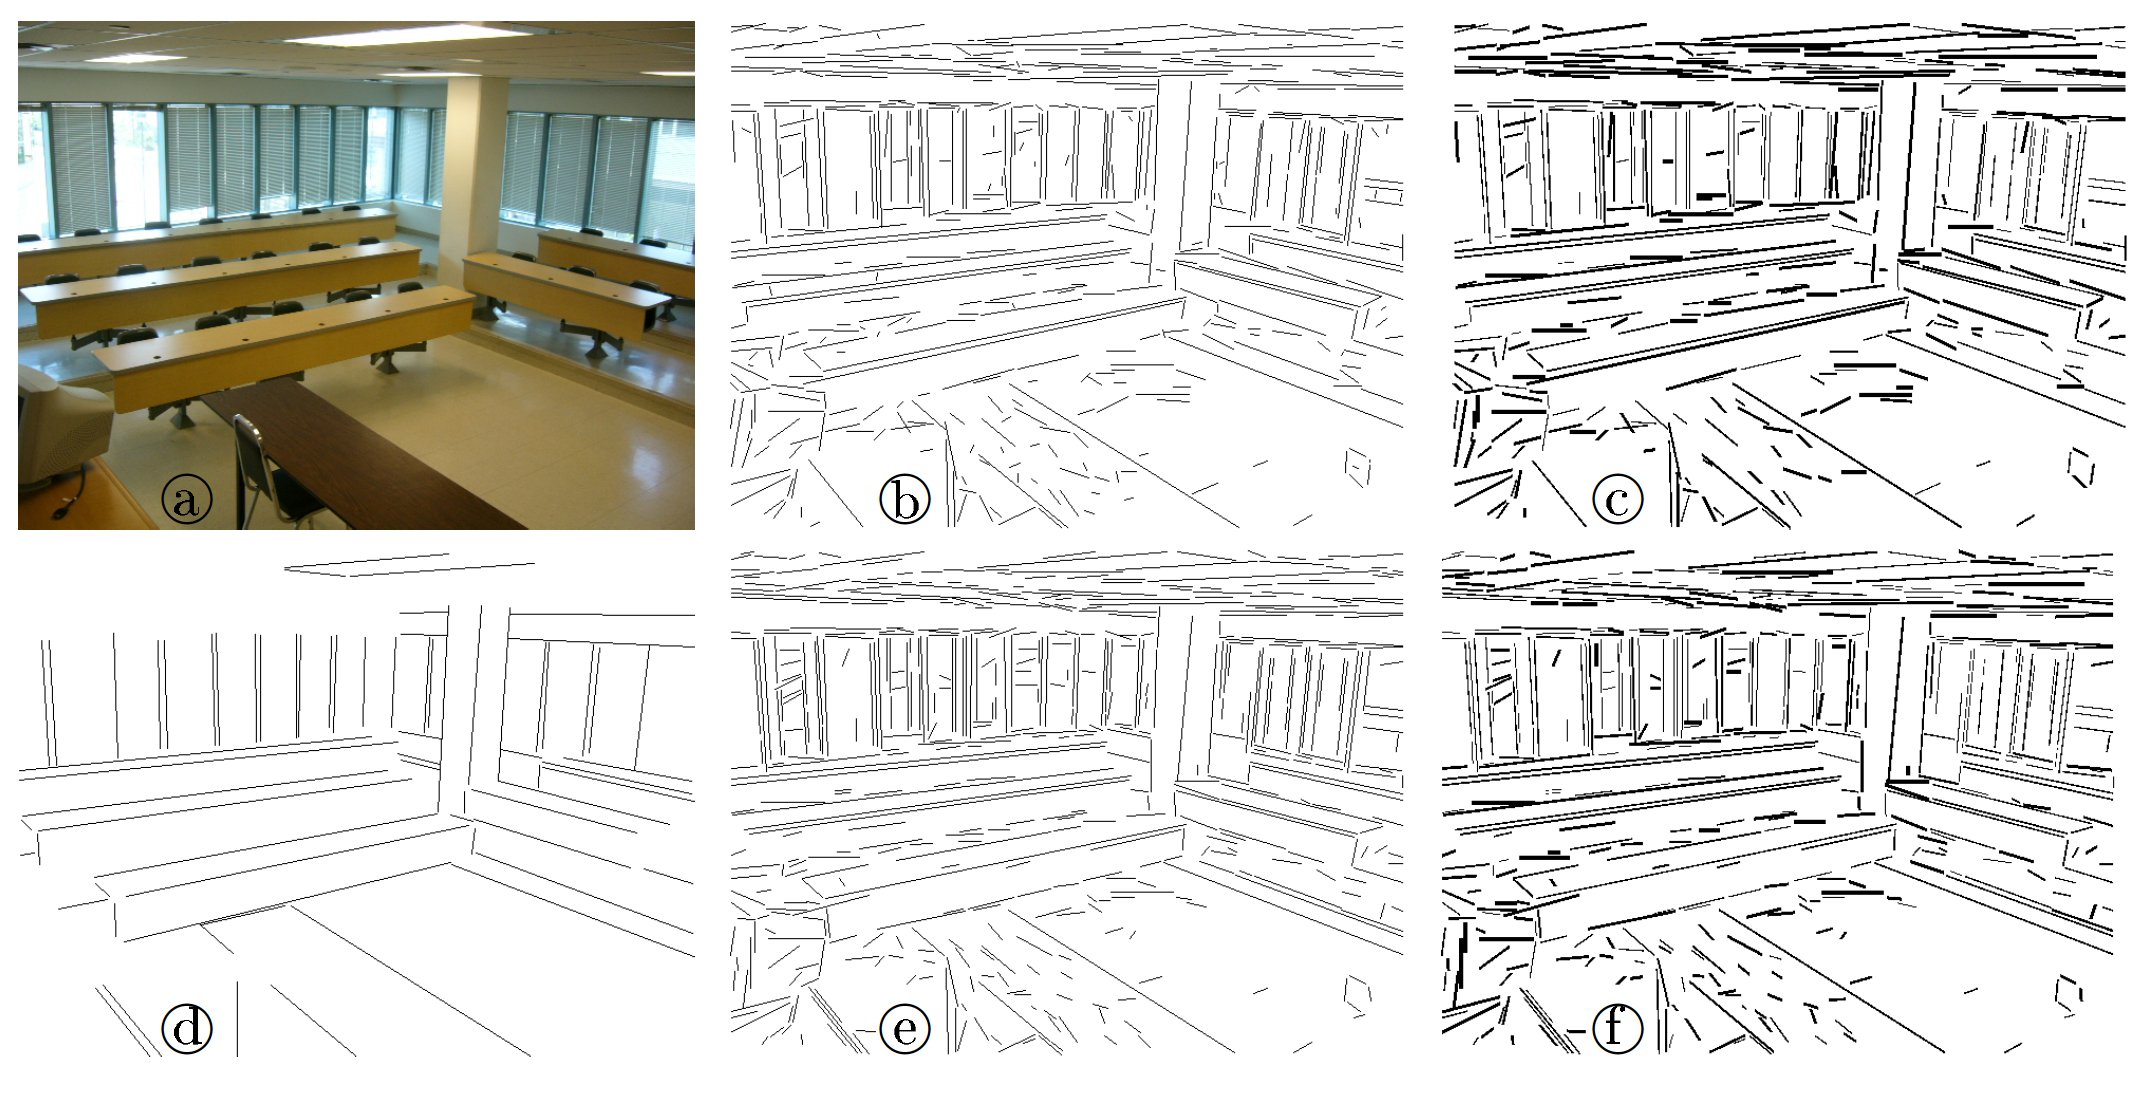
\includegraphics[width=0.95\textwidth]{Images/expe0.png}
  \end{center}
  \caption{Automatic detection on real images:
    P1020928 image from York Urban data base \cite{Denis08} (a),
    the associated groundtruth lines (d),
    the naive lines found without (b) and with (e) ADS and ATC concepts,
    the thick lines found without (c) and with (f) ADS and ATC concepts.}
  \label{fig:york}
\end{figure}



\begin{longtable}[]{l@{}|@{}c@{}c@{}c@{}c@{}c@{}}
\toprule
\begin{minipage}[b]{0.18\columnwidth}\raggedright
ADS \& ATC\strut
\end{minipage} & \begin{minipage}[b]{0.14\columnwidth}\centering
T (ms)\strut
\end{minipage} & \begin{minipage}[b]{0.14\columnwidth}\centering
C (\%)\strut
\end{minipage} & \begin{minipage}[b]{0.14\columnwidth}\centering
N\strut
\end{minipage} & \begin{minipage}[b]{0.14\columnwidth}\centering
L/N (pixels)\strut
\end{minipage} & \begin{minipage}[b]{0.14\columnwidth}\centering
W (pixels)\strut
\end{minipage}\tabularnewline
\midrule
\endhead
\begin{minipage}[t]{0.18\columnwidth}\raggedright
Without\strut
\end{minipage} & \begin{minipage}[t]{0.14\columnwidth}\centering
75.19 \textpm 16.60\strut
\end{minipage} & \begin{minipage}[t]{0.14\columnwidth}\centering
70.2 \textpm 10.1\strut
\end{minipage} & \begin{minipage}[t]{0.14\columnwidth}\centering
421 \textpm 98\strut
\end{minipage} & \begin{minipage}[t]{0.14\columnwidth}\centering
46.22 \textpm 8.60\strut
\end{minipage} & \begin{minipage}[t]{0.14\columnwidth}\centering
2.20 \textpm 0.16\strut
\end{minipage}\tabularnewline
\begin{minipage}[t]{0.18\columnwidth}\raggedright
With\strut
\end{minipage} & \begin{minipage}[t]{0.14\columnwidth}\centering
66.62 \textpm 15.47\strut
\end{minipage} & \begin{minipage}[t]{0.14\columnwidth}\centering
67.9 \textpm 9.6\strut
\end{minipage} & \begin{minipage}[t]{0.14\columnwidth}\centering
478 \textpm 111\strut
\end{minipage} & \begin{minipage}[t]{0.14\columnwidth}\centering
41.67 \textpm 7.53\strut
\end{minipage} & \begin{minipage}[t]{0.14\columnwidth}\centering
1.89 \textpm 0.13\strut
\end{minipage}\tabularnewline
\bottomrule  
\caption{Measure with and without ADS and ATC concepts on the
York Urban Database \cite{Denis08}.}
\label{tab:york}
\end{longtable}

\pagebreak


\begin{figure}
  \begin{center}
  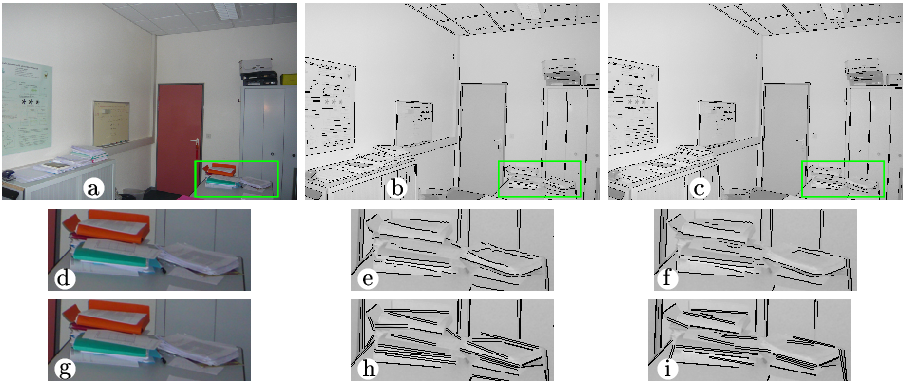
\includegraphics[width=0.95\textwidth]{Images/expe1.png}
  \end{center}
  \caption{Automatic detection on real images: 800x533 office image (a),
    the segments found without (b) and with (c) ADS and ATC concepts,
    a detail of the image (d,g),
    the points of detected blurred segments without (e) and with (f) ADS
    and ATC concepts and the bounding lines of detected blurred segments
    without (h) and with (i) ADS and ATC concepts.}
  \label{fig:office}
\end{figure}



\begin{longtable}[]{l|cccc}
\toprule
\begin{minipage}[b]{0.18\columnwidth}\raggedright
ADS \& ATC \strut
\end{minipage} & \begin{minipage}[b]{0.14\columnwidth}\centering
T (ms) \strut
\end{minipage} & \begin{minipage}[b]{0.14\columnwidth}\centering
N \strut
\end{minipage} & \begin{minipage}[b]{0.14\columnwidth}\centering
L/N (pixels) \strut
\end{minipage} & \begin{minipage}[b]{0.14\columnwidth}\centering
W (pixels) \strut
\end{minipage} \tabularnewline
\midrule 
Without & 48.16 & 254 & 53.92 & 1.99 \tabularnewline
With & 42.17 & 285 & 49.69 & 1.69 \tabularnewline
\bottomrule
\caption{Measure with and without ADS and ATC concepts on office image.}
\label{tab:office}
\end{longtable}

\pagebreak

\begin{figure}
  \begin{center}
  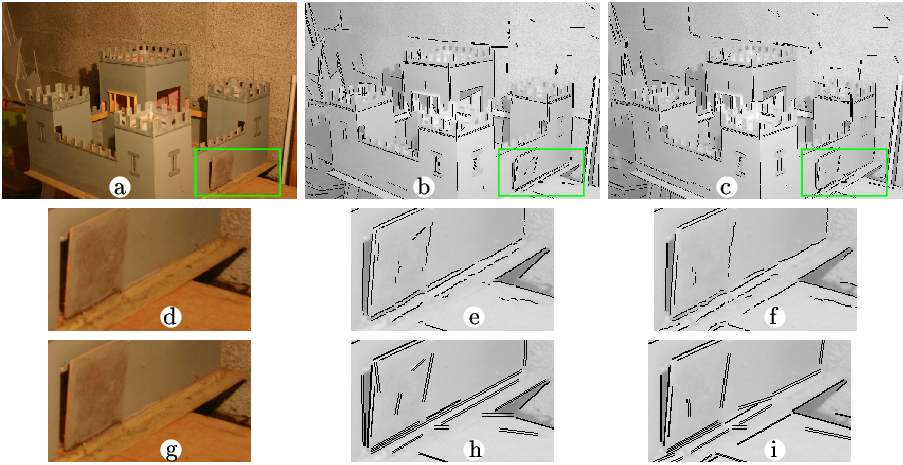
\includegraphics[width=0.95\textwidth]{Images/expe2.png}
  \end{center}
  \caption{Automatic detection on real images: 768x512 castle image (a), the segments found without (b) and with (c) ADS and ATC concepts, a detail of the image (d,g), the points of detected blurred segments without (e) and with (f) ADS and ATC concepts and the bounding lines of detected blurred segments without (h) and with (i) ADS and ATC concepts.}
\label{fig:castle}
\end{figure}


\begin{longtable}[]{l|cccc}
\toprule
\begin{minipage}[b]{0.18\columnwidth}\raggedright
ADS \& ATC \strut
\end{minipage} & \begin{minipage}[b]{0.14\columnwidth}\centering
T (ms) \strut
\end{minipage} & \begin{minipage}[b]{0.14\columnwidth}\centering
N \strut
\end{minipage} & \begin{minipage}[b]{0.14\columnwidth}\centering
L/N (pixels) \strut
\end{minipage} & \begin{minipage}[b]{0.14\columnwidth}\centering
W (pixels) \strut
\end{minipage} \tabularnewline
\midrule
Without & 104.30 & 361 & 36.58 & 2.23 \tabularnewline
With & 94.21 & 424 & 32.18 & 1.98 \tabularnewline
\bottomrule

\caption{Measure with and without ADS and ATC concepts on castle image.}
\label{tab:castle}
\end{longtable}


\bibliographystyle{plain}
\bibliography{ms}



\end{document}


